\documentclass[12pt]{article}
\usepackage{float}
\usepackage{booktabs}
\usepackage{tabulary}
\usepackage{svg}
\usepackage{tikz}
\usepackage{pgfplots}
\usepackage{indentfirst} %alinhar 1 parágrafo

\usepackage{sbc-template}
\usepackage{graphicx}
\usepackage{dirtytalk}

\usepackage[T1]{fontenc}
\usepackage{mathtools}
\usepackage{blkarray, bigstrut}
\usepackage{gauss}
\usepackage{amsmath}
\usepackage{afterpage}
\usepackage{graphicx,url}

%\usepackage[brazil]{babel}
\usepackage[utf8]{inputenc}

\pgfplotsset{compat=1.10}
\usetikzlibrary{%
    intersections,%
    arrows,%
    decorations.pathmorphing,%
    backgrounds,%
    positioning,%
    fit,%
    petri,%
    calc,%
    through,%
    graphs,%
    shapes.misc,%
    trees,%
    mindmap,%
    shadows,%
    calendar%
}

\sloppy

\title{Assessment of climate change impacts on hydro resources in Três Marias reservoir using machine learning models}

\author{%
    Bruno T. R. V. Silva\inst{1}, %
    Carolina S. Ansélmo\inst{1}, \\%
    Paula C. S. Borba\inst{1}, %
    Wallace S. S. Souza\inst{1}%
}

\address{%
    Department of Civil Engineering -- Aeronautics Institute of Technology\\
    São José dos Campos, Brazil
    \email{bruno.valeriano@ga.ita.br, carolina.anselmo@ga.ita.br}%
    \vspace{-2ex}
    \email{paula.borba@ga.ita.br,  wallace.souza@ga.ita.br}
%	\today
}


\begin{document}

\maketitle

%\begin{resumo}

%\end{resumo}

\section{Introduction}

Impacts of climate change on hydro resources have become a growing concern, since it may affect negatively the electricity supply in coming years, particularly in countries highly dependent on hydropower, like Brazil. Therefore, the ability to assess and make predictions about the water level and streamflow of reservoirs allows important decisions to be made by competent authorities in order to ensure that water resources can be appropriately allocated.

% TODO: preencher citação, transformar 'ONS (2020)' em citação
Over 63\% of the whole electricity supply in Brazil came from hydropower in 2019. However, Brazil faces reduced availability of hydro resources in recent years. ONS affirmed that Brazil is experiencing a drought period similar to the period between 1948 to 1955 \cite{onsseca}, while other studies suggested the occurrence of more frequent and anomalous droughts in Brazil due to climate changes.

% TODO: No final do paragrafo, talvez seja bom elencar os estudos que sugerem uma frequência anormal
Climate change may affect hydroelectric production mainly because of the precipitation altering. Reduced precipitation may compromise river flows, while increased precipitation could render a power plant unproductive as it could exceed its capacity. Also, the increase in average temperature may alter the soil moisture level, interfering with the flow and storage of water in dams \cite{Mukheibir2013}. According to \cite{Lyra2018}, southeastern Brazil will suffer a significant reduction of precipitation during the twenty-first century. While \cite{Queiroz2016} noted that the Southeast may be benefited from climate changes with considerable increases in electricity generation, but in other regions of Brazil, climate change will likely cause the reduction of hydroelectricity production.

Global Climate Models (GCMs) simulate interactions of climate systems based on physical principles and observational data. They are tools that are used to predict weather patterns and to explore climate sensitivities in scenarios of climate change \cite{gcm}. To provide long-term simulations of climate change at higher resolution, GCMs are downscaled to Regional Climate Models (RCMs), which include projections at a higher resolution.
This study explored the impact of two climate change scenarios,  Representative Concentration Pathway (RCP 4.5 and RCP 8.5), on hydro resources in the Três Marias reservoir, located in the Southeast of Brazil.

Thus, the objective of this article is to make a forecast of the flow and water level of a reservoir using machine learning predictive models. The dataset come from a simulation of the Platform Project of the Center for Weather Forecasting and Climate Studies (CPTEC) of the National Institute for Space Research (INPE). The simulated input data using will be (i) precipitation, (ii) evaporation, (iii) temperature, and (iv) surface runoff. As output data, the water level and stream flow of the reservoir.

\section{Related bibliography}

As pointed by \cite{ardabili2019deep}, using physical or statistical models to study hydrological processes can raise several problems, such as high computational costs, weakness in uncertainty analysis and the need for a large amount of comprehensive data. Therefore, the usage of machine learning methods have been growing among research community, as shown in Figure~\ref{fig:num_publications}, as a strategy to tackle some of these problems.
In addition, several researchers have used machine learning to predict hydrological patterns, such as to predict flow in future hydrographic basins considering climate changes \cite{bhatta2019evaluation}, daily flow to river \cite{kassem2020predicting}, and flow of the hydroelectric plant reservoir \cite{essenfelder2020smart}. Table~\ref{tab:variables-literature} shows the variables used in these studies.

\begin{figure}[htb]
    \centering
    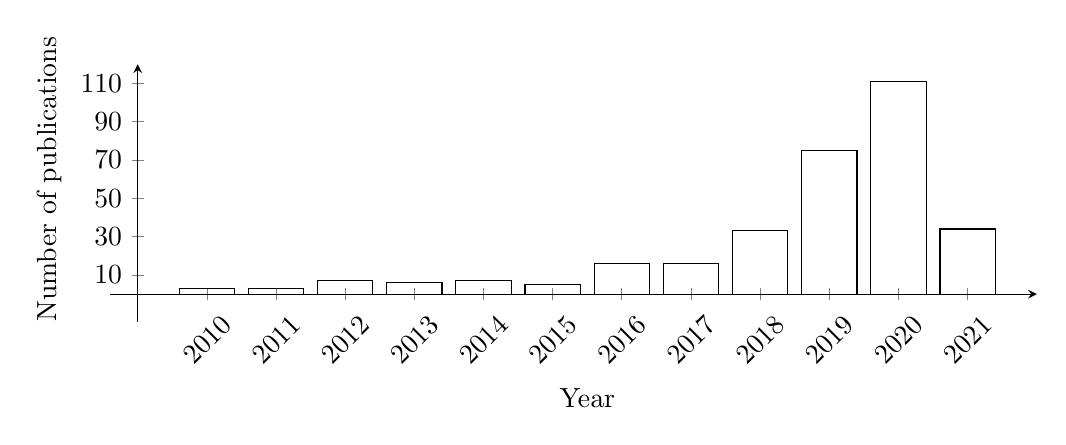
\begin{tikzpicture}
        \begin{axis}[
                width=13cm,
                height=4.5cm,
                style={/pgf/number format/set thousands separator={}},
                axis x line=bottom,
                axis y line=left,
                axis line style={shorten <=-10},
                xmin=2009,
                xmax=2022,
                xtick={2010,...,2021},
                ymin=0,
                ymax=120,
                ytick={10, 30,...,110},
                xlabel={Year},
                xticklabel style={rotate=45},
                ylabel={Number of publications}
            ]
            \addplot[black,ybar,fill, fill opacity=0.0, bar width = 0.8] table {
                2021    34
                2020    111
                2019    75
                2018    33
                2017    16
                2016    16
                2015    5
                2014    7
                2013    6
                2012    7
                2011    3
                2010    3
            };
        \end{axis}
    \end{tikzpicture}
    \caption{Number of publications about machine learning applied in the study of hydrological processes. The search string used was ``\texttt{(Machine learning) AND (hydrological))}'' in the Engineering Village database}
    \label{fig:num_publications}
\end{figure}

\begin{table}[htbp]
\centering
\caption{Variables in the related bibliograpy}
\label{tab:variables-literature}
    \begin{tabulary}{\textwidth}{lCCC}
        \toprule
           & Kassem et al (2019) & Bhatta et al (2019) & Essenfelder et al (2020) \\
        \midrule
            Precipitation & X & X & X \\
            Temperature & X & X & X \\
            Relative humidity & X &  & \\
            Wind speed  & X &  & \\
            Landuse classes  &  & X & \\
            Stream flow  & X & X & X \\
        \bottomrule
    \end{tabulary}
\end{table}

\cite{kicsi2007streamflow} presented a comparison between four different neural networks algorithms applied in short term daily stream flow forecast. They concluded that the Levenberg–Marquardt algorithm, when compared with backpro pagation, conjugate gradient and cascade correlation takes a relatively small time for training, while giving the best stream flow forecast, even using correlation analysis as the method to determine the input vector. Concurrently, \cite{petty2018streamflow} assessed the capacity of employing machine learning techniques and big data to impute streamflow using historical and real-time data. Their results demonstrated that applying Streamflow Hydrology Estimate using Machine Mearning (SHEM) models could be used to estimate streamflow and even to help fill missing data from historical datasets.

\section{Material and methods}
Using two different scenarios, RCP 4.5 and RCP 8.5, we explored the long-term effect of climate variables on flow and water level variables. The predictor and outcome variables are described in Figure~\ref{fig:approach}.

\begin{figure}[htbp]
  \centering
  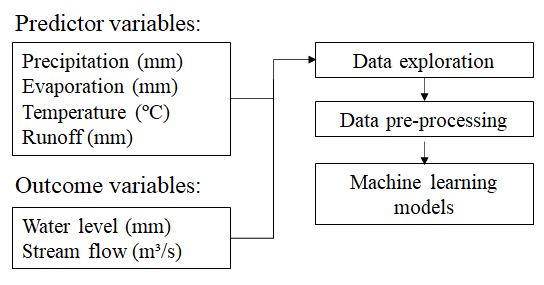
\includegraphics[width=0.5\linewidth]{Figures/approach.png}
  \caption{Methodology}
  \label{fig:approach}
\end{figure}

\subsection{Descriptive analysis}
We chose Três Marias reservoir for two main reasons. First because of its importance to the Brazilian electricity system, since this reservoir holds a hydropower plant of 396 MW of installed capacity. Second, there are available climate data at a high spatial resolution (5 km) for the Southeastern region, where Três Marias is located. Três Marias reservoir is inside the Alto São Francisco sub-basin in Minas Gerais state (Figure \ref{fig:studyarea}).

\begin{figure}[htbp]
  \centering
  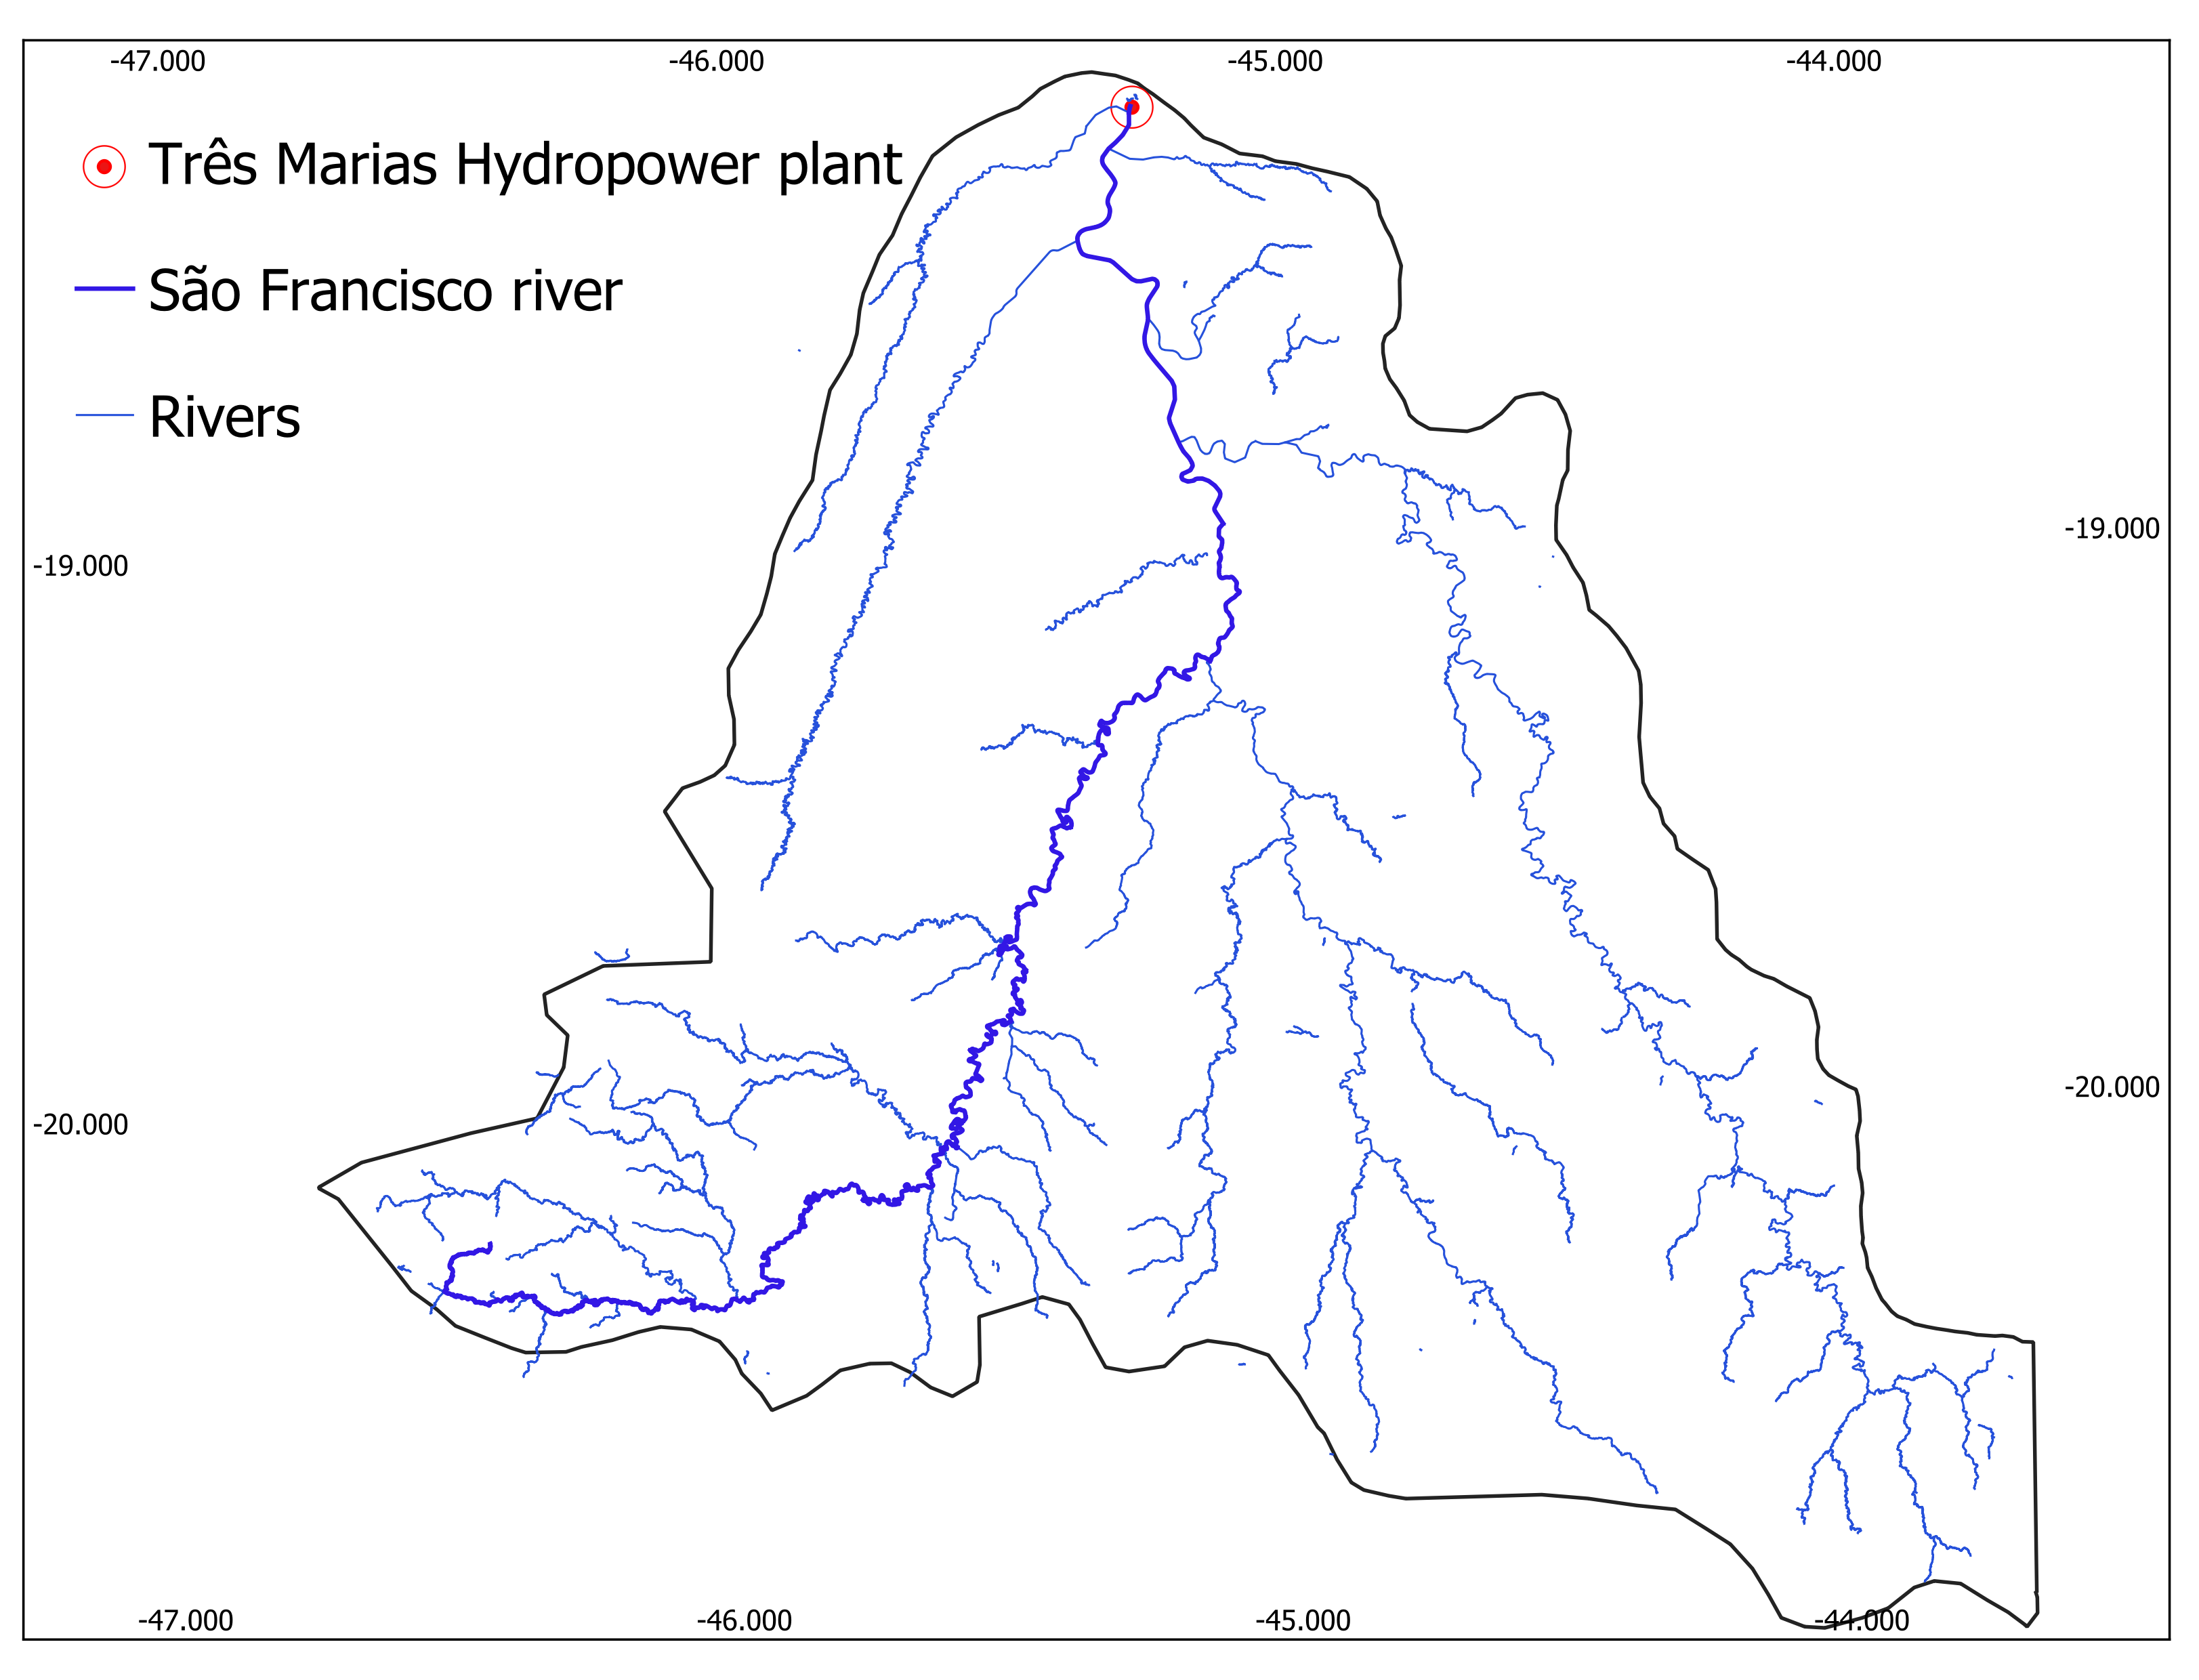
\includegraphics[width=0.6\linewidth]{Figures/mapa_v0.png}
  \caption{Alto São Franscisco sub-basin.}
  \label{fig:studyarea}
\end{figure}

In order to reduce the complexity, we opted to use the contribution of each river and sub-basin area to the stream flow and water level from \cite{fundep}. Thus, we made an manual classification from all coordinates to 11 points based in the distance to the nearest river which represents the area of influence (Figure \ref{fig:coord}).

\begin{figure}[htbp]
  \centering
  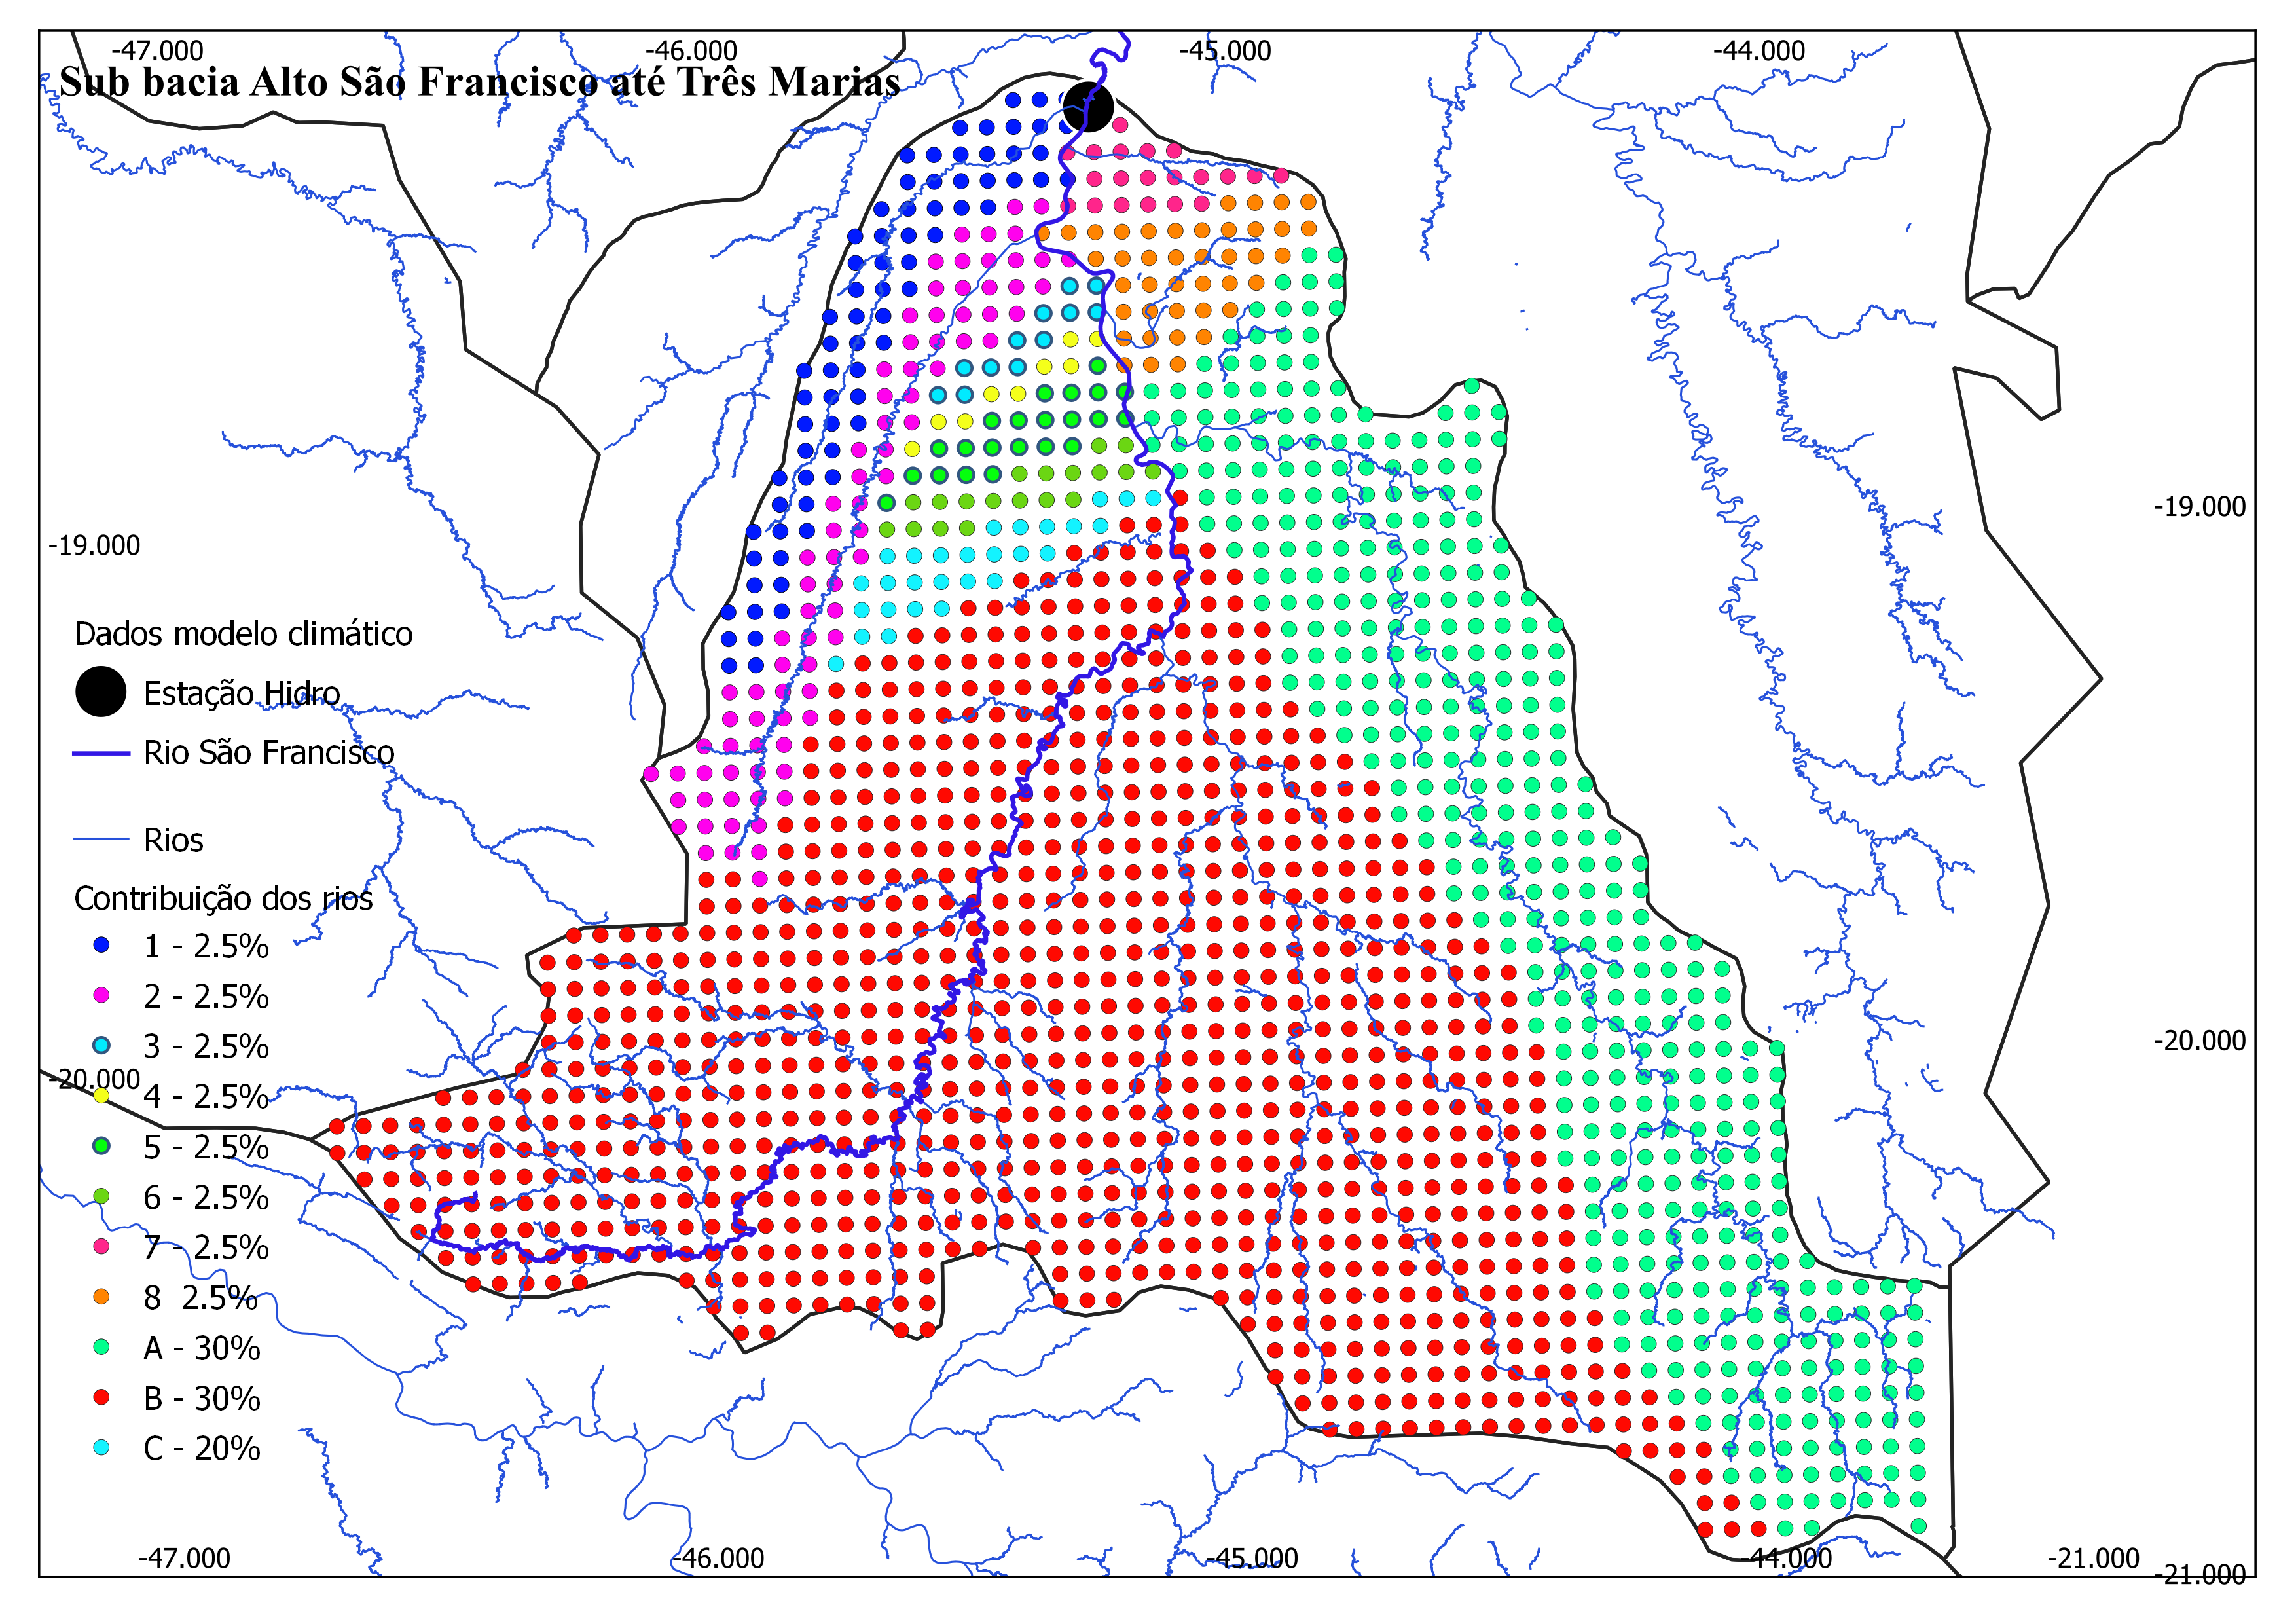
\includegraphics[width=0.6\linewidth]{Figures/coord_contribuicao.png}
  \caption{Coordinate points and their contribution rate.}
  \label{fig:coord}
\end{figure}

\subsection{Data}
In order to apply machine learning to forecast streamflow and water level for Três Marias reservoir, we used data generated by CPTEC/INPE and made available on the Projeta Platform \cite{chou2014assessment,chou2014evaluation,Lyra2018}. This data is split into historic observations, ranging from January, 1961 to December, 2005 and projections modeled according to RCP 4.5 and RCP 8.5, ranging from January, 2006 to December, 2099. For our study, since observations of flow and water levels for Três Marias reservoir made available by ONS \cite{onsnivel,onsvazao} start in 1999, historical data collected from the Projeta platform were filtered to start at the same period.

A list of potential predictors is shown in Table~\ref{tab:predictors}. The study area, Alto São Francisco sub-basin, was subdivided in 1672 equally sized regions, and for each of these regions, data regarding temperature, precipitation, evaporation and surface runoff were gathered, according to temporal resolution, historical data and modeled projections shown in Table~\ref{tab:predictors}, which lists the potential predictors alongside to their respective measurement units. Additionally, Table~\ref{tab:outcomes} shows the measurement units, temporal resolution and date range for data regarding streamflow and water level for the Três Marias reservoir.

\begin{table}[htbp]
\centering
\caption{Relation of predictors considered in this study obtained on the Projeta Platform \cite{chou2014assessment,chou2014evaluation,Lyra2018}}
\label{tab:predictors}
    \resizebox{0.8\columnwidth}{!}{%
    \begin{tabulary}{\textwidth}{lcCcCr}
        \toprule
            Variable       & Unit & Temporal resolution & Historical data & Modeled Projections \\
        \midrule
            Temperature (T)    & ºC   & Daily               & 1999-2005       & 2006-2099 \\
            Precipitation (P) & mm   & Daily               & 1999-2005       & 2006-2099 \\
            Evaporation (E)    & mm   & Daily               & 1999-2005       & 2006-2099 \\
            Surface runoff (R) & mm   & Daily               & 1999-2005       & 2006-2099 \\
        \bottomrule
    \end{tabulary}
    }
\end{table}

\begin{table}[htbp]
    \centering
    \caption{Outcome variables made available by ONS \cite{onsnivel,onsvazao}}
    \label{tab:outcomes}
    \resizebox{0.6\columnwidth}{!}{%
    \begin{tabular}{lccr}
        \toprule
            Variable       & Unit & Temporal resolution & Historical data \\
        \midrule
            Streamflow (SF)           & m³/s & Daily               & 1999-2021 \\
            Water level (WL)    & m    & Daily               & 1999-2021 \\
        \bottomrule
    \end{tabular}
    }
    \label{tab:my_label}
\end{table}

%Descrever os dados: números de exemplos, de atributos, os tipos e escalas dos atributos, se é classificação/regressão, etc.. Se for classificação, dizer a proporção de exemplos na classe com mais observações (majoritária).

%\subsection{Técnicas}

%\section{Results}\label{sec:figs}

% Precisamos citar: Integração de dados (merges), Eliminação de atributos e como tratamos valores fora da faixa (RNOF) e limpeza de dados (verificar)

\section{Data preprocessing}

In order to organize the data into attribute-value format, we followed three main steps: data reduction, data integration and data transformation. Originally, we had a large dataset with the variables P, E, T and R related to 1673 coordinate points inside the sub-basin limits in the period between 1999 to 2005.

We aggregated the coordinate points into 11 groups of rivers according to their contribution area to the Três Marias reservoir and removed information that are not necessary to the model, such as the latitude and longitude (Figure \ref{fig:step1}).

Then, in order to reduce the original dataset and transform it into the information that represents all points in their respective group, we considered the daily sum for P and E, and the daily mean for T and R values (Figure \ref{fig:step2}). Thus, we created weather variables of P, E, T and R for 11 groups of rivers instead of 1673 points.

Although time is an important feature relating to weather variability, we did not consider the date as an attribute, since the seasonal changes are already incorporated in the magnitude of the other variables.

\begin{figure}[htbp]
  \centering
  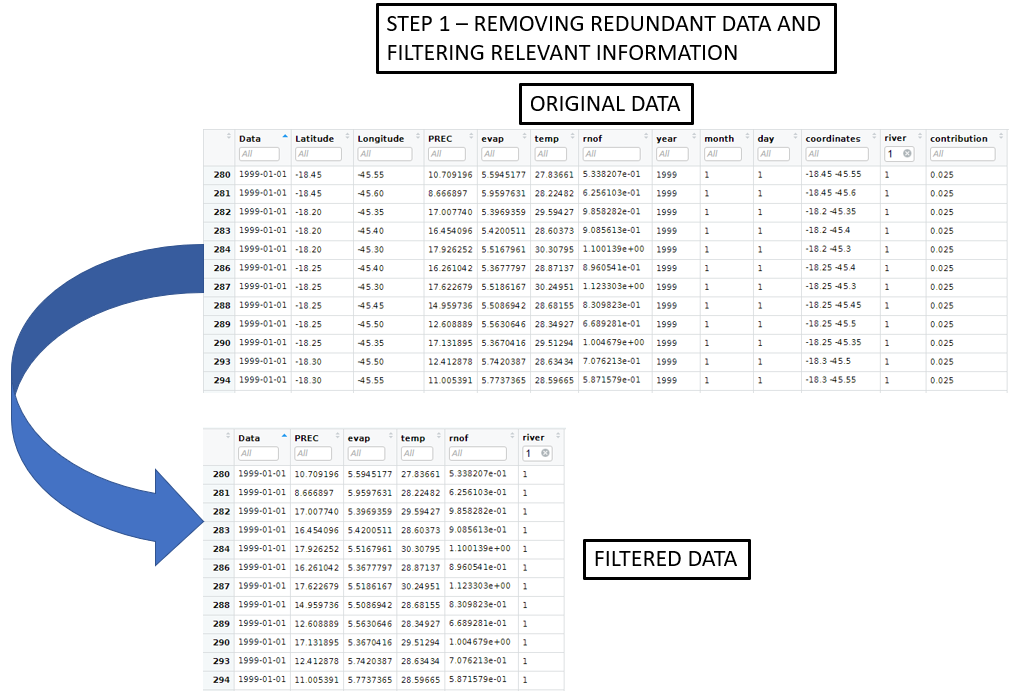
\includegraphics[width=1\linewidth, trim=0cm 0 0 2.2cm,clip=true]{Figures/STEP1.png}
  \caption{Step 1: data reduction.}
  \label{fig:step1}
\end{figure}

\begin{figure}[htbp]
  \centering
  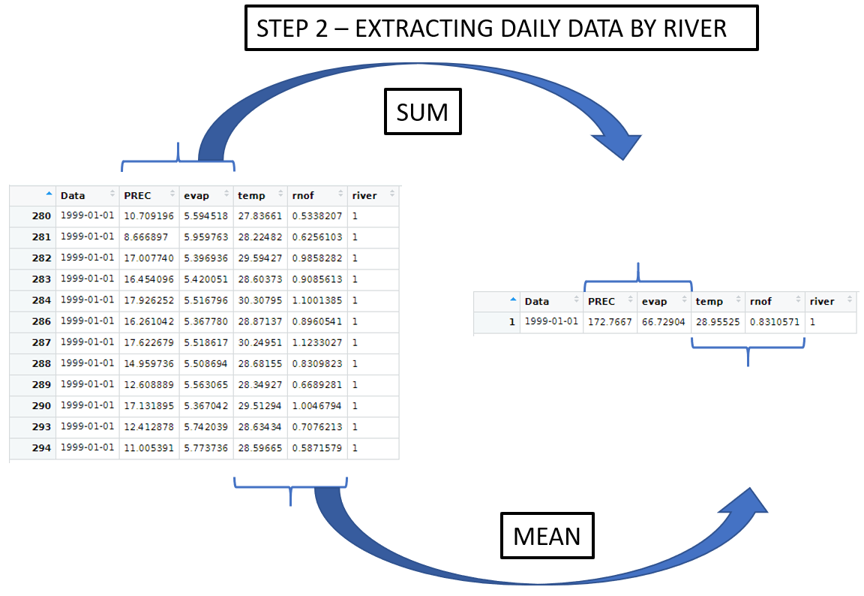
\includegraphics[width=1\linewidth, trim=0cm 0 0 1.5cm,clip=true]{Figures/STEP2.png}
  \caption{Step 2: feature aggregation.}
  \label{fig:step2}
\end{figure}

In data integration, we combined three different databases. Here, we joined weather variables (predictors) with Water Level (WL) and Stream-Flow (SF), which are both features related to the Três Marias reservoir (Figure \ref{fig:step3}). Besides that, they are the target variables. The mathematical representation of merging databases is illustrated in Figure \ref{fig:matriz1}. Finally, we obtained the data matrix in attribute-value format, which is represented in Figure \ref{fig:matriz2}.

\begin{figure}[htbp]
  \centering
  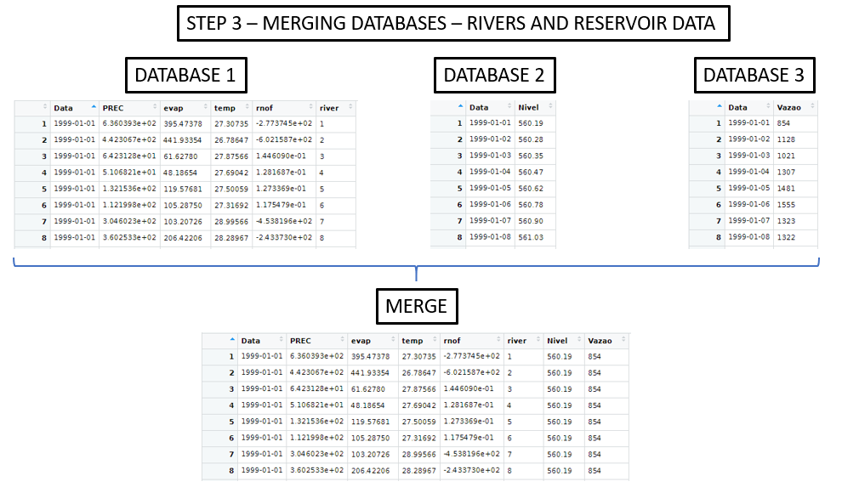
\includegraphics[width=1\linewidth, trim=0cm 0 0 1.2cm,clip=true]{Figures/STEP3.png}
  \caption{Step 3: data integration.}
  \label{fig:step3}
\end{figure}

\begin{figure}[htbp]
  \centering
  \[
  \setlength{\arraycolsep}{0pt}% No column separation in array; manual spacing
                               % by supplying empty groups {} around operators
  \renewcommand{\arraystretch}{1.5}% Stretch out content vertically
  \resizebox{.7\textwidth}{!}{
  $
  \begin{array}{ *{8}{c} }
    % Header row in \scriptstyle
    \scriptstyle Database \: 1 & & % +
    \scriptstyle Database \: 2 & & % +
    \scriptstyle Database \: 3 & & & % =
     \\
    % Matrix/vector row
    \begin{blockarray}{ccccccc}
    & P & E & T & R & River \\
    \begin{block}{c[cccccc]}
    Day_1 & a_{1,1}&a_{1,2}&a_{1,3}&a_{1,4}&1\bigstrut[t] \\
    Day_1 & a_{2,1}&a_{2,2}&a_{2,3}&a_{2,4}&2 \\
    \vdots & \vdots & \vdots & \vdots & \vdots & \vdots\\
    Day_1 & a_{11,1}&a_{11,2}&a_{11,3}&a_{11,4}&c \\
    Day_2 & a_{12,1}&a_{12,2}&a_{12,3}&a_{12,4}&1 \\
    \vdots & \vdots & \vdots & \vdots & \vdots & \vdots\\
    Day_n & a_{n,1}&a_{n,2}&a_{n,3}&a_{n,4}&c \\
    \end{block}
    \end{blockarray}\vspace*{-1.25\baselineskip}
    & {} + {} &
    \begin{blockarray}{cccccc}
    & WL \\
    \begin{block}{c[ccccc]}
    Day_1 & a_{1,1}\bigstrut[t] \\
    Day_2 & a_{2,1} \\
    Day_3 & a_{3,1} \\
    Day_4 & a_{4,1} \\
    Day_5 & a_{5,1} \\
    \vdots & \vdots \\
    Day_n & a_{n,1}\bigstrut[b]\\
    \end{block}
    \end{blockarray}\vspace*{-1.25\baselineskip}
    & {} + {} &
    \begin{blockarray}{cccccc}
    & SF \\
    \begin{block}{c[ccccc]}
    Day_1 & a_{1,1}\bigstrut[t] \\
    Day_2 & a_{2,1} \\
    Day_3 & a_{3,1} \\
    Day_4 & a_{4,1} \\
    Day_5 & a_{5,1} \\
    \vdots & \vdots \\
    Day_n & a_{n,1}\bigstrut[b]\\
    \end{block}
    \end{blockarray}\vspace*{-1.25\baselineskip}
  \end{array}
  $
  }
\]
  %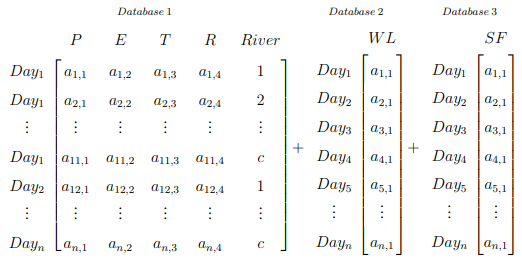
\includegraphics[width=1\linewidth]{Figures/matriz1.png}
  \caption{Matrix of different databases}
  \label{fig:matriz1}
\end{figure}



\begin{figure}[htbp]
  \centering
  \[
  \setlength{\arraycolsep}{0pt}% No column separation in array; manual spacing
                               % by supplying empty groups {} around operators
  \renewcommand{\arraystretch}{1.5}% Stretch out content vertically
  \resizebox{.8\textwidth}{!}{
  $
  \begin{array}{ *{8}{c} }
    % Header row in \scriptstyle
    \scriptstyle Attribute-value \: database % +
     \\
    % Matrix/vector row
    \begin{blockarray}{ccccccccccccccccc}
    & P_1 & \cdots & P_c & E_1 & \cdots & E_c  &
    T_1 & \cdots & T_c & T_1 & \cdots & T_c & WL & SF
    \\
    \begin{block}{c[cccccccccccccccc]}
    Day_1 & a_{1,1}&\cdots&a_{1,11}&
    a_{1,12} & \cdots &a_{1,22} &
    a_{1,23} & \cdots &a_{1,33} &
    a_{1,34} & \cdots &a_{1,44} &
    a_{1,45} & a_{1,46}
    \bigstrut[t] \\

    Day_2 & a_{2,1} &\cdots&a_{2,11}&
    a_{2,12} & \cdots &a_{2,22} &
    a_{2,23} & \cdots &a_{2,33} &
    a_{2,34} & \cdots &a_{2,44} &
    a_{2,45} & a_{2,46}
    \\

    \vdots & \vdots & \cdots & \vdots & \vdots &
    \cdots & \vdots & \vdots &
    \cdots & \vdots & \vdots &
    \cdots & \vdots & \vdots & \vdots
    \\

    Day_n & a_{n,1}&a_{n,3}&a_{n,4}&
    a_{n,12} & \cdots & a_{n,22} &
    a_{n,23} & \cdots &a_{n,33} &
    a_{n,34} & \cdots &a_{n,44} &
    a_{n,45} & a_{n,46}
    \\
    \end{block}
    \end{blockarray}%\vspace*{-1.25\baselineskip}
  \end{array}
  $
  }
\]

  %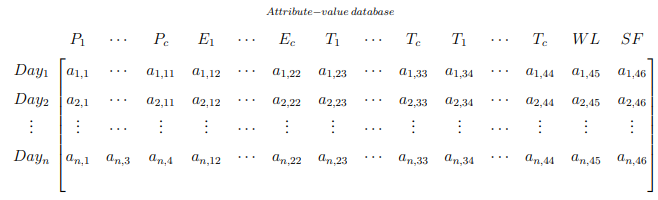
\includegraphics[width=1\linewidth]{Figures/matriz2.png}
  \caption{Data matrix}
  \label{fig:matriz2}
\end{figure}

\subsection{Normalization}
The results of the earlier procedures indicate there's values in multiple scales in the dataset. Since the prediction model selected in the next steps can be sensitive to scale features, we normalized the data with the min-max normalization with the mathematical equation represented in \ref{eqn:Normalization}:
\begin{equation}
\label{eqn:Normalization}
x' = \frac{x-min(x)}{max(x)-min(x)}
\end{equation}
where ~$x$ is the present value, ~$min(x)$ is the minimum value of the feature and ~$max(x)$ is the maximum value of the feature.

We applied this procedure for every variable in the dataset. While only the scale in the values changed with the normalization procedure, it is easier to identify the variation in mean and standard deviation between variables, as shown in Figure \ref{fig:Normalized} for the inputs in the first river.

\begin{figure}[htbp]
  \centering
  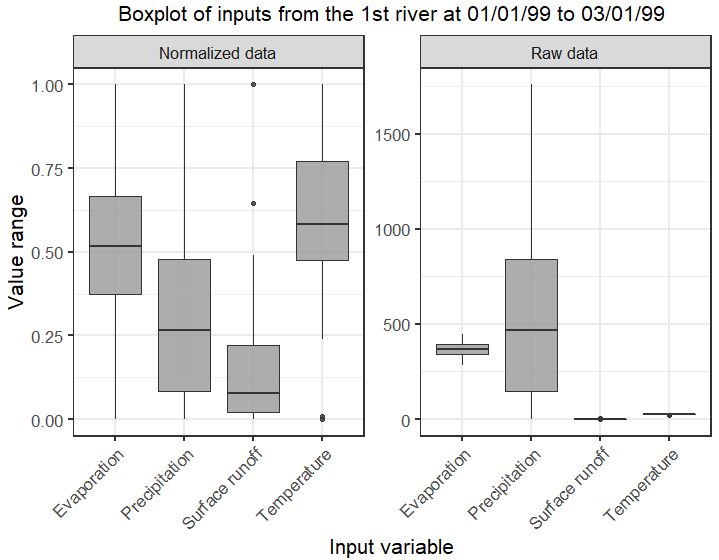
\includegraphics[width=0.6\linewidth, trim=0cm 0 0 .7cm,clip=true]{Figures/Normalização.png}
  \caption{Boxplot of inputs from raw data x normalized data}
  \label{fig:Normalized}
\end{figure}

Other preprocessing procedures, such as feature selection or dimensionality reduction, are not applicable since we filtered the data in the first step (download from Projeta Platform). Therefore, all data is composed of numeric values that make other transformation techniques unnecessary.

In the future, we intend to verify if the variation between measures can generate better results for the prediction model than absolute values, such as comparison between reservoir levels and variation between days.

In conclusion, we converted the database in the format attribute-value with normalized values between features. The "CSV" file extension archive in the annex provides further information about the newly generated dataset.

%\subsection{Machine learning models} \label{subsec:pre-processamento}

%Parte a ser entregue até o dia 21/06.

%\section{Discussion}

%Discutir os resultados obtidos. Parte a ser entregue até o dia 21/06.

%\section{Conclusion}

\bibliographystyle{sbc}
\bibliography{sbc-template}

\end{document}
